\chapter{Nástroje pre sieťovú virtualizáciu}

Čo je:
EVE-ng, GNS3, Dynamips, VIRL 

Odkiaľ je, čím sa vyznačuje, ako sa ovláda

Prieskum dostupných virtualizačných nástrojov + súčasný stav na katedre.

\section{Motivácia}
- Dôvody, prečo použiť virtuálne laboratóriá.

  Je to tu nutné dávať, keď som sa tomu venoval v Úvode a v Cieľoch práce?
  
\section{Porovnávacie kritériá}

Pri porovnávaní jednotlivých virtuálnych sieťových laboratórii som sa rozhodoval podľa nasledovných kritérii:
\begin{itemize}
    \item Použité vývojové technológie
    \item Podpora zariadení, s ktorými sa na danom predmete pracuje
    \item Podpora technológií jednotlivých zariadení
    \item Typ používateľského rozhrania
    \item Prideľovanie portových čísel zariadeniam
    \item Vzdialený prístup ku zariadeniam (telnet, vnc, rdp)
    \item Vytvorenie/úprava/uloženie/odstránenie topológie
    \item Počet topológii, ktoré môže mať jeden používateľ spustených
    \item Možnosť práce viac ľudí naraz na rovnakom projekte
    \item Možnosť prepojiť topológiu so živou sieťou
\end{itemize}


\section{Dostupné riešenia}

\subsection{Dynamips/Dynagen}

Dynamips je emulátor Cisco smerovačov \cite{dynamips}. Nástroj je v prevažnej mierie napísaný v jazyku C \cite{dynamips_github}. Podporuje iba výlučne vybrané Cisco smerovače \cite{dynamips}. V súčasnosti sa používa na katedre pri výučbe predmetov Projektovanie sietí 1 a CCNP Routing. Ovláda sa cez príkazový riadok. Portové čísla na vzdialený prístup sa zariadeniam prideľujú manuálne. Vzdialený prístup k zariadeniam v topológii je realizovaný protokolom \emph{telnet}. Na vytváranie topológii sa používa jednoduchý značkovací jazyk. Nástroj Dynagen, ktorý slúži ako nadstavba nad platformou Dynamips, slúži na jednoduchšiu prácu s topológiami \cite{dynamips}. Topológie môže spravovať výlučne administrátor, pretože ani Dynamips, ani Dynagen nevedia rozlišovať rôzne typy používateľov. Počet topológii, ktoré môžu byť súčasne spustené je obmedzené iba výkonom servera. Na jednej topológii môžu pracovať aj viacerí študenti, tým že sa rozdelia portové čísla zariadení v topológii medzi študentov. Nástroj Dynamips umožňuje prepojiť topológiu so živou sieťou \cite{dynamips, dynamips_nil}. Na obrázku \ref{obr:dynamips_dynagen} je znázornený nástroj Dynagen.

\begin{figure}
    \centering
    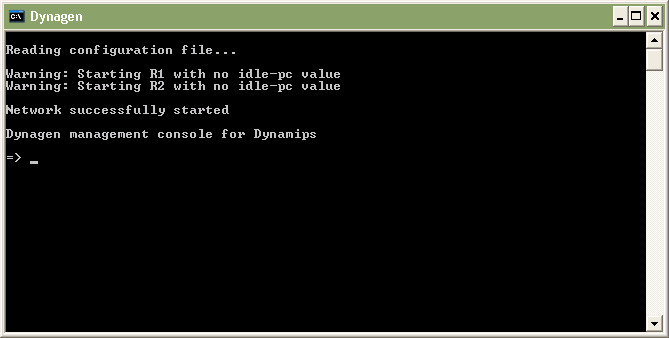
\includegraphics[width=0.75\textwidth]{dynamips_dynagen}
    \caption{Nástroj Dynagen spustený v prostredí Windows} \cite{obr_dynamips_dynagen}
    \label{obr:dynamips_dynagen}
\end{figure}

\subsection{WEB-IOU}



\subsection{Cisco VIRL}

\subsection{VIRO}

Projekt Petra Hadača.

\subsection{UNetLab}

\subsection{EVE-ng}

popis + rozdiely rôznych verzií (špeciálne pre EVE-ng) - PRIMÁRNE! + rozdiely vo funkcionalitách podľa tabuľky na oficiálnej stránke EVE-ng.

\subsection{GNS3}

- podporný nástroj

\section{Vyhodnotenie}

Porovnanie GNS3 a EVE-ng.

Odôvodnenie, prečo som si vybral práve EVE-ng.